\section{System Design} 
\label{section:design_and_implementation}

In this chapter a novel system design is proposed to tackle the requirements highlighted in the previous chapter and bring SSI concepts to this use case. This will start with a decision on the technologies to use for the different components of the system, followed by a presentation of a generic SSI with IoT system topology. After this, the Verifiable Electric Vehicle Charging system's architecture with SSI will be described.

\subsection{Technological Decisions}

In this section the decisions and rationales for the technologies to use for this project will be presented. In Table~\ref{tab:final_tech_stack} a summary is provided for the decisions taken for each aspect of the technology stack. In the sections to follow the rationale for these decisions is presented, mentioning relevant literature and the prime aspects considered when assessing the Distributed Ledger to use and consequently which network to select, and the best solutions available regarding agent implementations.

\begin{table}[!htb]
    \centering
    \begin{tabular}{|c|c|}
    \hline
        \textbf{Technology} & \textbf{Decision} \\
        \hline
         Distributed Ledger & \textit{Hyperledger Indy} \\
         Network Selection & \textit{BCovrin Test Indy Network} \\
         Agent & \textit{Hyperledger Aries Cloud Agent - Python (ACA-Py)} \\
         Mobile Agent & \textit{Trinsic Wallet}\\
         \hline
    \end{tabular}
    \caption{List of decisions on technologies to be adopted for the proposed solution}
    \label{tab:final_tech_stack}
\end{table}

\subsubsection{Distributed Ledger}
\label{subsubsec:distributed_Ledger}

In this chapter the motivation for the selected framework will be made, picking up on the foundations laid by Table~\ref{tab:frameworks}, where an overview of the existing SSI frameworks was presented according to the literature. By following the discussion in Section~\ref{subsec:existing_technologies_and_application_domains}, the decision on which framework to use was narrowed down to Hyperledger Indy or the IOTA Tangle. Most of the quality attributes listed in Section~\ref{subsubsec:key_drivers} are satisfied by both Hyperledger Indy\footnote{\url{https://github.com/hyperledger/indy-sdk}} and IOTA\footnote{\url{https://github.com/iotaledger/identity.rs}}, so it is relevant to assess where these diverge to make a decision on which framework to utilize.

\begin{table}[!ht]
    \centering
    \begin{threeparttable}[h]
        \centering
        \begin{tabular}{|p{36mm}|cc|}
        \hline
             \backslashbox[40mm]{Considerations}{Frameworks} & Hyperledger Indy & IOTA Tangle\\
             \hline
             Active Development & + & +\\
             Decentralized IdMS & + & +\\
             Permissioned & + & -\\
             Transaction Costs & + & =\\
             Open-Source & + & + \\
             Support for SSI & + & + \\
             Easy-to-find Resources & + & -\\
             Open-Source Agents & + & =\\
             Easy-to-Deploy & + & =\\
             Standardization & + & =\\
             \hline
        \end{tabular}
        \begin{tablenotes}
        \item The "+", "=", "-" icons demonstrate that the framework is a good, neutral (not enough information) or bad solution, respectively, regarding a given aspect.
        \end{tablenotes}
    \end{threeparttable}
    \caption{Pros and Cons of Hyperledger Indy compared to IOTA Tangle}
    \label{tab:technological_decision}
\end{table}

Looking at the aspects described in Table~\ref{tab:technological_decision}, it is possible to see that Indy is favorable in the aspects considered in that table. 

One aspect which was discussed in Section~\ref{subsec:existing_technologies_and_application_domains} is that in order to provide an SSI-based IoT solution, the selected framework used and its underlying DLT implementation need to be analyzed with respect to the access protocol used (permissioned or permissionless) \cite{luecking2020decentralized}.
When analyzing the literature one of the main reasons why the adoption of Indy was made at the detriment of IOTA \cite{zhu2018identity} was due to the permissioned nature of the first, which cuts down any transaction costs \cite{lo2019analysis}.

\paragraph{Decision}

Indy is based on the Hyperledger ecosystem, which offers more standardization compared to the rest of the frameworks available.
Aside from that, Indy provides one aspect which others do not: the fact that no public data is written on the ledger, which strengthens the security and privacy of the system.
At last, given that Indy has a continuous support and has a very active community at the time of writing, and that it offers itself as a solution for the digital identity use case, it will be the framework used in this project.\\

\paragraph{Choice of Network}

Whilst deciding on the Hyperledger Indy DLT ensures the technology to use for the blockchain component of this system, there are different networks to use, and depending on the requirements of the system, a choice needs to be made.

Deploying a network of Indy nodes manually is a laborious task that suffers from lack of documentation. As an alternative to this, a project called \acrfull{VON}\footnote{\label{vonx}\url{https://vonx.io/}}, contributed by the Province of British Columbia already exists. The latter allows to mitigate the aforementioned issue by not only providing the means to deploy a portable development level Indy Node network, but also the maintainers have already-deployed networks which are possible to use. The rationale for this project mentions that \textit{"The Verifiable Organizations Network (VON) is a community effort to establish a better way to find, issue, store and share trustworthy data about organizations—locally and around the globe. Community partners are using jointly developed software components to enable the digitization of government-issued public credentials—registrations, permits, and licenses. Currently, VON components are based on Hyperledger Indy distributed ledger technology"}\footref{vonx}.

The decision to use a network provided by this project aligns with the needs of the proposed solution, since its components are based on the Indy DLT as mentioned before. 

Therefore, there are three alternatives for using this projects networks:

\begin{itemize}
    \item Local Deployment of the VON Network\footnote{\url{https://github.com/bcgov/von-network}}
    \item Use the already-deployed BCovrin Test Indy Network (Ideal for Proof-of-Concepts)\footnote{\url{http://test.bcovrin.vonx.io/}}
    \item Use the already-deployed BCovrin Prod Indy Network (Ideal for stable production-level solutions)\footnote{\url{http://prod.bcovrin.vonx.io/}}
\end{itemize}

At an early stage of the development it is possible to use a local deployment of the VON network, since it is good for making tests on connecting agents and issuing credentials. The reason for this is that if an error is committed (wrong transaction is put in the ledger for example), the network can be brought down and restarted with ease.

%However, given that it is meant for the network to allow connection between all agents, there is a constraint as to which networks the agents support.

\paragraph{Decision}

Given that this study ultimately aims at developing a proof-of-concept as the means of evaluating the proposed system architecture, the BCovrin Test Network would be ideal. If this project reaches a production state, it is possible to move to the BCovrin Prod Indy Network.

\subsubsection{Agent Technology}
\label{subsubsec:agent_technology}

Following the description of what agents are in Section~\ref{subsubsec:wallets_and_agents}, a decision on which agent to use and its implementation needs to be made.
The decision will mostly be between using an open-source agent built using the Hyperledger Aries framework or creating an agent from scratch using existing libraries and resources available.

At the time of writing, the most widely used agents are created under the Hyperledger Aries framework concepts. The choice for which agents to use needs alignment with the adopted DLT, which in the case of this system is Hyperledger Indy. The goal for Hyperledger Aries agents is to become blockchain-agnostic. This means that the aim is that for SSI-related implementations the usage of these agents are not restricted to Hyperledger Indy's blockchain. However, at the time of writing, there is only support for Hyperledger Indy, which complies with the aforementioned decisions regarding the DLT.

The Hyperledger Aries agents are essentially a piece of software that allow for any entity to assume any role in the Verifiable Credentials Model (Section~\ref{subsubsec:verifiable_credential_model}) and allows the entities to interact with each other, whilst also creating an environment capable of handling verifiable credential exchange. 

The core components of an Aries agent are demonstrated in Figure~\ref{fig:aries_agent_architecture}. Here it is possible to see four different components: the Key Management Service, which will handle the private and public keys; the Agent Messaging Interface, which will handle communication with other agents; the Ledger Interface, to directly communicate with the ledger; and at last the controller, which can be programmed according to the given use case.

\begin{figure}[!htb]
    \centering
    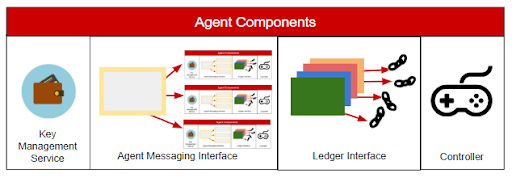
\includegraphics[width=0.7\linewidth]{images/Agent_Components.png}
    \caption[Aries Agent Architecture]{Aries Agent Architecture\protect \footnotemark}
    \label{fig:aries_agent_architecture}
\end{figure}

\footnotetext{\url{https://courses.edx.org/assets/courseware/v1/acc3247dbf74b710586a75f0854699ab/asset-v1:LinuxFoundationX+LFS172x+3T2019+type\@asset+block/Agent_Components.png}}

For this project the agents that will be used are the \acrfull{ACA-Py} implementation. According to the development team, "\textit{ACA-Py is built on the Aries concepts and features that make up Aries Interop Profile (AIP) 1.0, as well as many of the protocols that will be in AIP 2.0. ACA-Py’s supported Aries protocols include, most importantly, protocols for issuing, verifying, and holding VCs that work with a Hyperledger Indy distributed ledger and the Indy "AnonCreds" credential format. Contributors are actively working on adding support for other ToIP Layer 1 DID Utilities, and for other VC formats.}"\footnote{\url{https://github.com/hyperledger/aries-cloudagent-python}}.
At the time of writing, the project has a very active community with constant updates and implementation of Aries \glspl{RFC} to accommodate to the standards adopted for SSI (whether Hyperledger standards or ones by W3C).

The ACA-Py agents expose a variety of \acrfull{REST} endpoints, that when hit, will spark an action that can range from connecting to another agent, issue a credential, revoke a credential, and many others. These are all documented when deploying an ACA-Py agent, presented using SwaggerUI\footnote{Software used to visualize and interact with the API’s resources - \url{https://swagger.io/tools/swagger-ui/}}, allowing for an easy way to interact with the agents and be mindful of the necessary parameters for specific actions (for example a credential object needs to be attached to the specific POST request for issuing a credential).

An important aspect to consider when thinking of selecting an agent implementation is whether it supports mediation or not. In the context of agents, mediation is needed in two scenarios: when agents are not guaranteed to be online 100\% of the time, or when the agents do not want to have their Public DIDs written to the ledger (for privacy reasons), which leaves them without an endpoint for other agents to connect to. In those events, there should be a mediator agent acting similar to an inbox for e-mail, that stores incoming messages and sends them as soon as the offline agent is back online, addressing the first scenario. 
When the mediated agent connects to other agents via a pairwise DID communication, the endpoint of the mediated agent will appear to the agent it connects to as the one from its mediator, resolving the second scenario.
Mediation is facilitated within the Hyperledger ACA-Py agent, making it a strong agent implementation regarding this aspect.
The mediator is never aware of the final recipient of the messages, nor about the content of the message, since onion routing is baked-in the current implementation of the agents, allowing the solution to benefit from higher privacy measures.

% \paragraph{Other Agent Implementations} An agent can be tailored for each solution, which means that for the literature that was consulted, for example Terzi et al. \cite{terzi2020securing}, a close-source agent was used in the different agents. This restricts the number of open-source components that can be used to create an agent.

\paragraph{Decision}

Given the fact that the ACA-Py agent is at a stage where it can be used for the majority of actions regarding SSI (establish connections, issue and handle credentials, revocation, mediation, etc), is open-source and has a Ledger Interface compatible with Hyperledger Indy (the Distributed Ledger adopted as highlighted in Section~\ref{subsubsec:distributed_Ledger}), it will be the agent implementation used in the solution.

\subsubsection{Mobile Agent}
\label{subsubsec:mobile_agent}

At the time of writing there are several implementations for mobile agents (also mentioned as wallets), which are meant to be used by the individuals on their mobile devices. These offer an already defined logic for controlling the actions regarding handling connections to other agents and how to use verifiable credentials to verify proof requests. One limitation regarding mobile agents is that they do not have a specific endpoint for other agents to connect to. Instead they require an agent (which can be running in the cloud) to act as its mediator. Mediation is a mechanism which will be explained in Section~\ref{subsubsec:architecture_of_the_system}.

The current agents that support Self-Sovereign Identity, identified from literature and online research are: Lissi\footnote{\url{https://lissi.id/}}, eSatus\footnote{\url{https://esatus.com/}}, Trinsic\footnote{\url{https://trinsic.id/}} and Connect.me\footnote{\url{https://www.connect.me/}}. There is also the Aries Mobile Agent Xamarin\footnote{\url{https://github.com/hyperledger/aries-mobileagent-xamarin}} which is an open-source project hosted under Hyperledger ecosystem. 

Although in this case the Xamarin agent would be a solution within the same ecosystem (Hyperledger), it is not yet mature enough for testing, while the Trinsic Wallet agent offers a ready-to-use solution, that has the possibility to connect to any Hyperledger Indy Network. This last statement indicates that this agent implementation complies with the choice for the selected network (BCovrin Test Indy Network), which has been adopted following the reasons mentioned in Section~\ref{subsubsec:distributed_Ledger}. Additionally, the Trinsic Wallet agent offers under-the-hood support for mediation, satisfying a privacy concern that will be described ahead.

\paragraph{Decision}

For the reasons mentioned in this section, the Trinsic Wallet App has been adopted as part of the proposed solution for the Mobile Agents' implementation.

\subsection{Architecture for SSI with IoT}
\label{subsec:architecture_for_ssi_with_iot}

In this section an overview of a generic solution for a system which uses SSI applied to IoT devices is presented. In Figure~\ref{fig:general_architecture_ssi_with_iot} a diagram illustrates the solution which is generic and highlights the necessary components for a system which has: 
\begin{itemize}
    \item Enterprise agents (presented in \textcolor{blue}{\textbf{blue}} on the left side as Entity A, B and C); 
    \item Mobile agents (in \textcolor{red}{\textbf{red}}) and its need for a mediator agent (in \textcolor{purple}{\textbf{purple}});
    \item IoT devices which are resource constrained (in need of a static agent);
    \item IoT devices that are not resource constrained.
\end{itemize}

In a general solution designed for SSI with IoT, the necessary components are:

\begin{itemize}
    \item A Distributed Ledger to store the DID registry, schemas, credential definitions and revocation registries, as mentioned in Section~\ref{subsec:what_information_goes_onto_the_DLT?};
    \item Agents running on behalf of each entity with pre-configured logic on how to interact between each other;
    \item For the logic of which actions are to be performed by the agents it is necessary to have a controller which will vary depending on the given use case;
    \item It is also possible that the agents have a webpage running in front of the controller, which provides a User Interface (UI) to manage interactions with the agent.
\end{itemize}

In the diagram represented in Figure~\ref{fig:general_architecture_ssi_with_iot} there are three different types of agents which have already been discussed in Section~\ref{subsubsec:wallets_and_agents}, \ref{subsubsec:agent_technology} and \ref{subsubsec:mobile_agent}. There are the Edge and Cloud agents as well as the Mobile agents. 

A point worth reflecting on in this section is the fact that some agents should not have a public DID available in the ledger (for example the agents that represent individuals or IoT devices). In these events, the mediator is necessary to provide a routing path between these agents and the outside world. 
The Mobile Agent will need the mediator agent as mentioned previously, with said mediator running in the cloud. 
This mediation is also observed in Figure~\ref{fig:general_architecture_ssi_with_iot} since there are mediators present for the Resource-Constrained IoT devices as well as Private-Non-Resource IoT devices.



\begin{figure}[!htb]
    \centering
    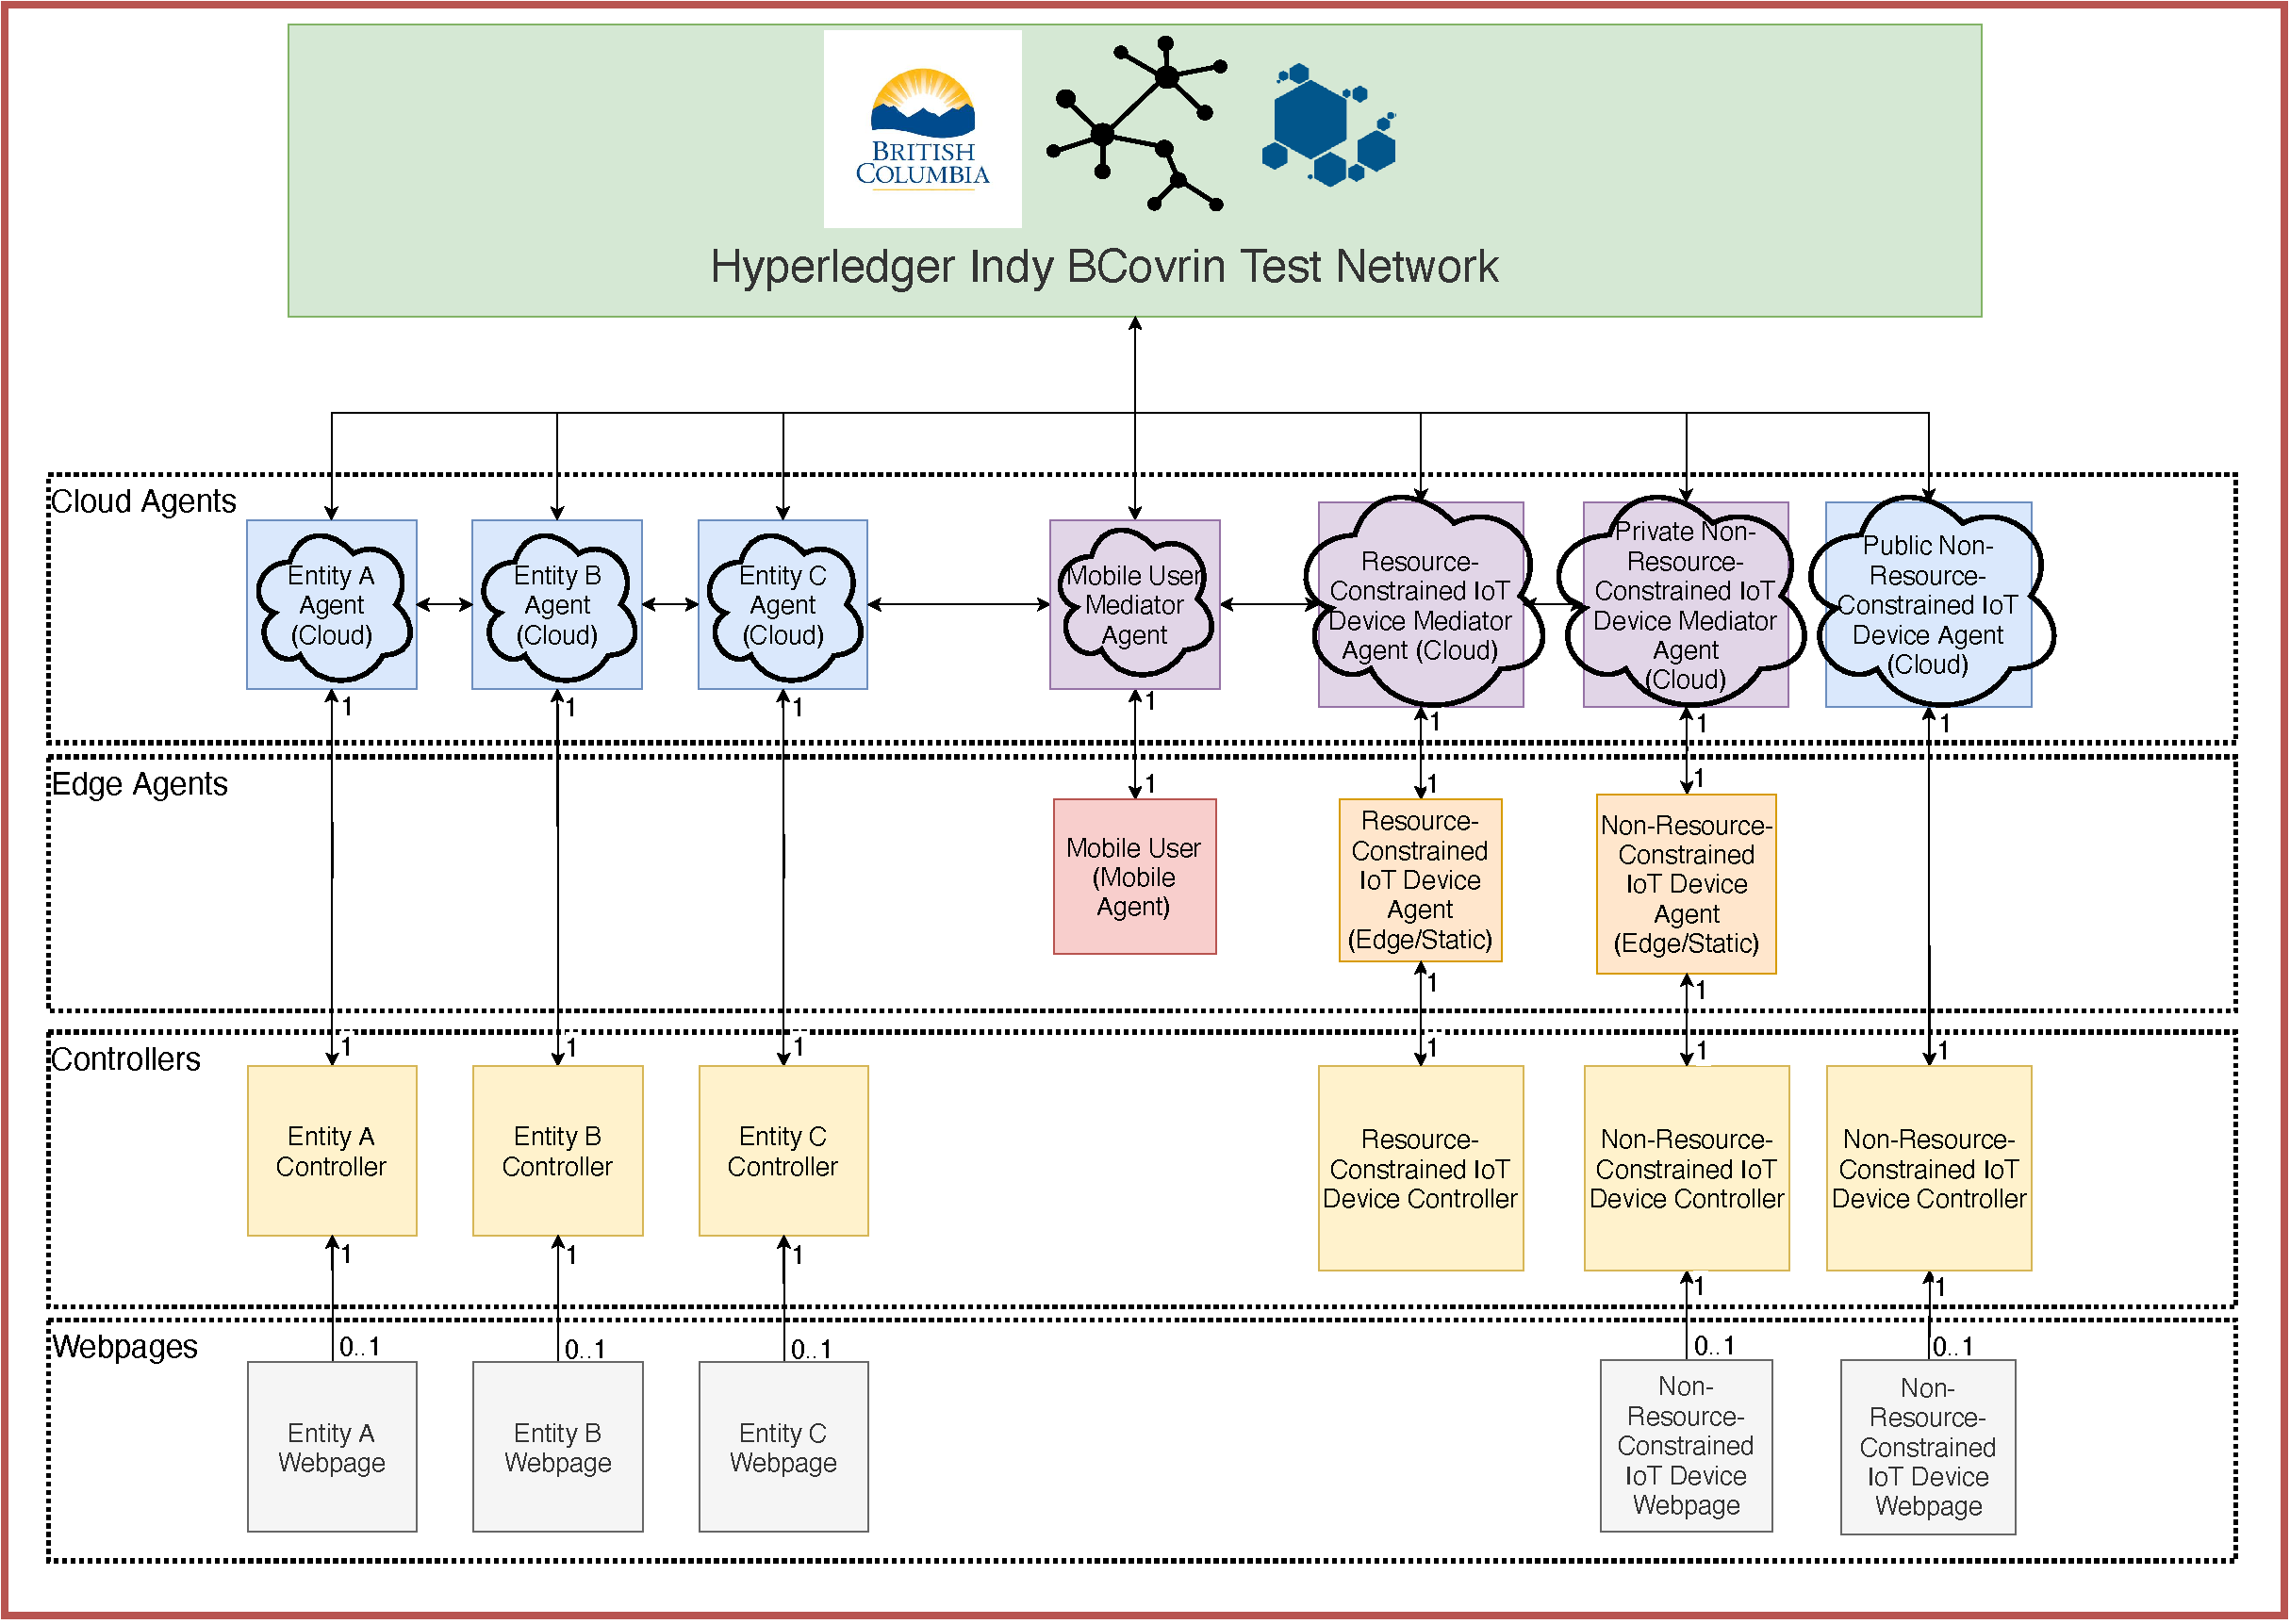
\includegraphics[width=0.85\linewidth]{images/SSIWithIoTArchitecture.pdf}
    \caption{General Architecture for SSI with IoT}
    \label{fig:general_architecture_ssi_with_iot}
\end{figure}

\newpage

\subsection{Electric Vehicle Charging System with SSI}
\label{subsec:architecture_for_electric_vehicle_charging_system_with_ssi}

For the design of the system to-be, the idea is to port the core concepts of the architecture presented in the general SSI with IoT design in Section~\ref{subsec:architecture_for_ssi_with_iot} into the architecture of the Electric Vehicle Charging System. This has to be done while still having in mind the core functionality for authentication of users and vehicles on this system, as presented earlier in Section~\ref{subsec:case_description}.

In this section a run-down of the flow of the system and its components will be presented, with focus on the interactions made between the agents, the different assumptions made, as well as a rationale for the decisions taken that combined into the proposed architecture. This is explained in detail in Section~\ref{subsubsec:architecture_of_the_system}. A detailed analysis on the mapping between real-life credentials and the Verifiable Credentials in the proposed architecture is made in Section~\ref{subsubsec:schemas_and_CDs}. The different flows present in this system and their specific use cases are illustrated in Section~\ref{subsubsec:information-flows-ssi}. A brief description of how each flow is ported to the new system is made. Additionally, for each use case description the agent interactions are highlighted with the appropriate level of detail, describing each party's role in the communication and the different assumptions made.

\begin{figure}[!htb]
    \centering
    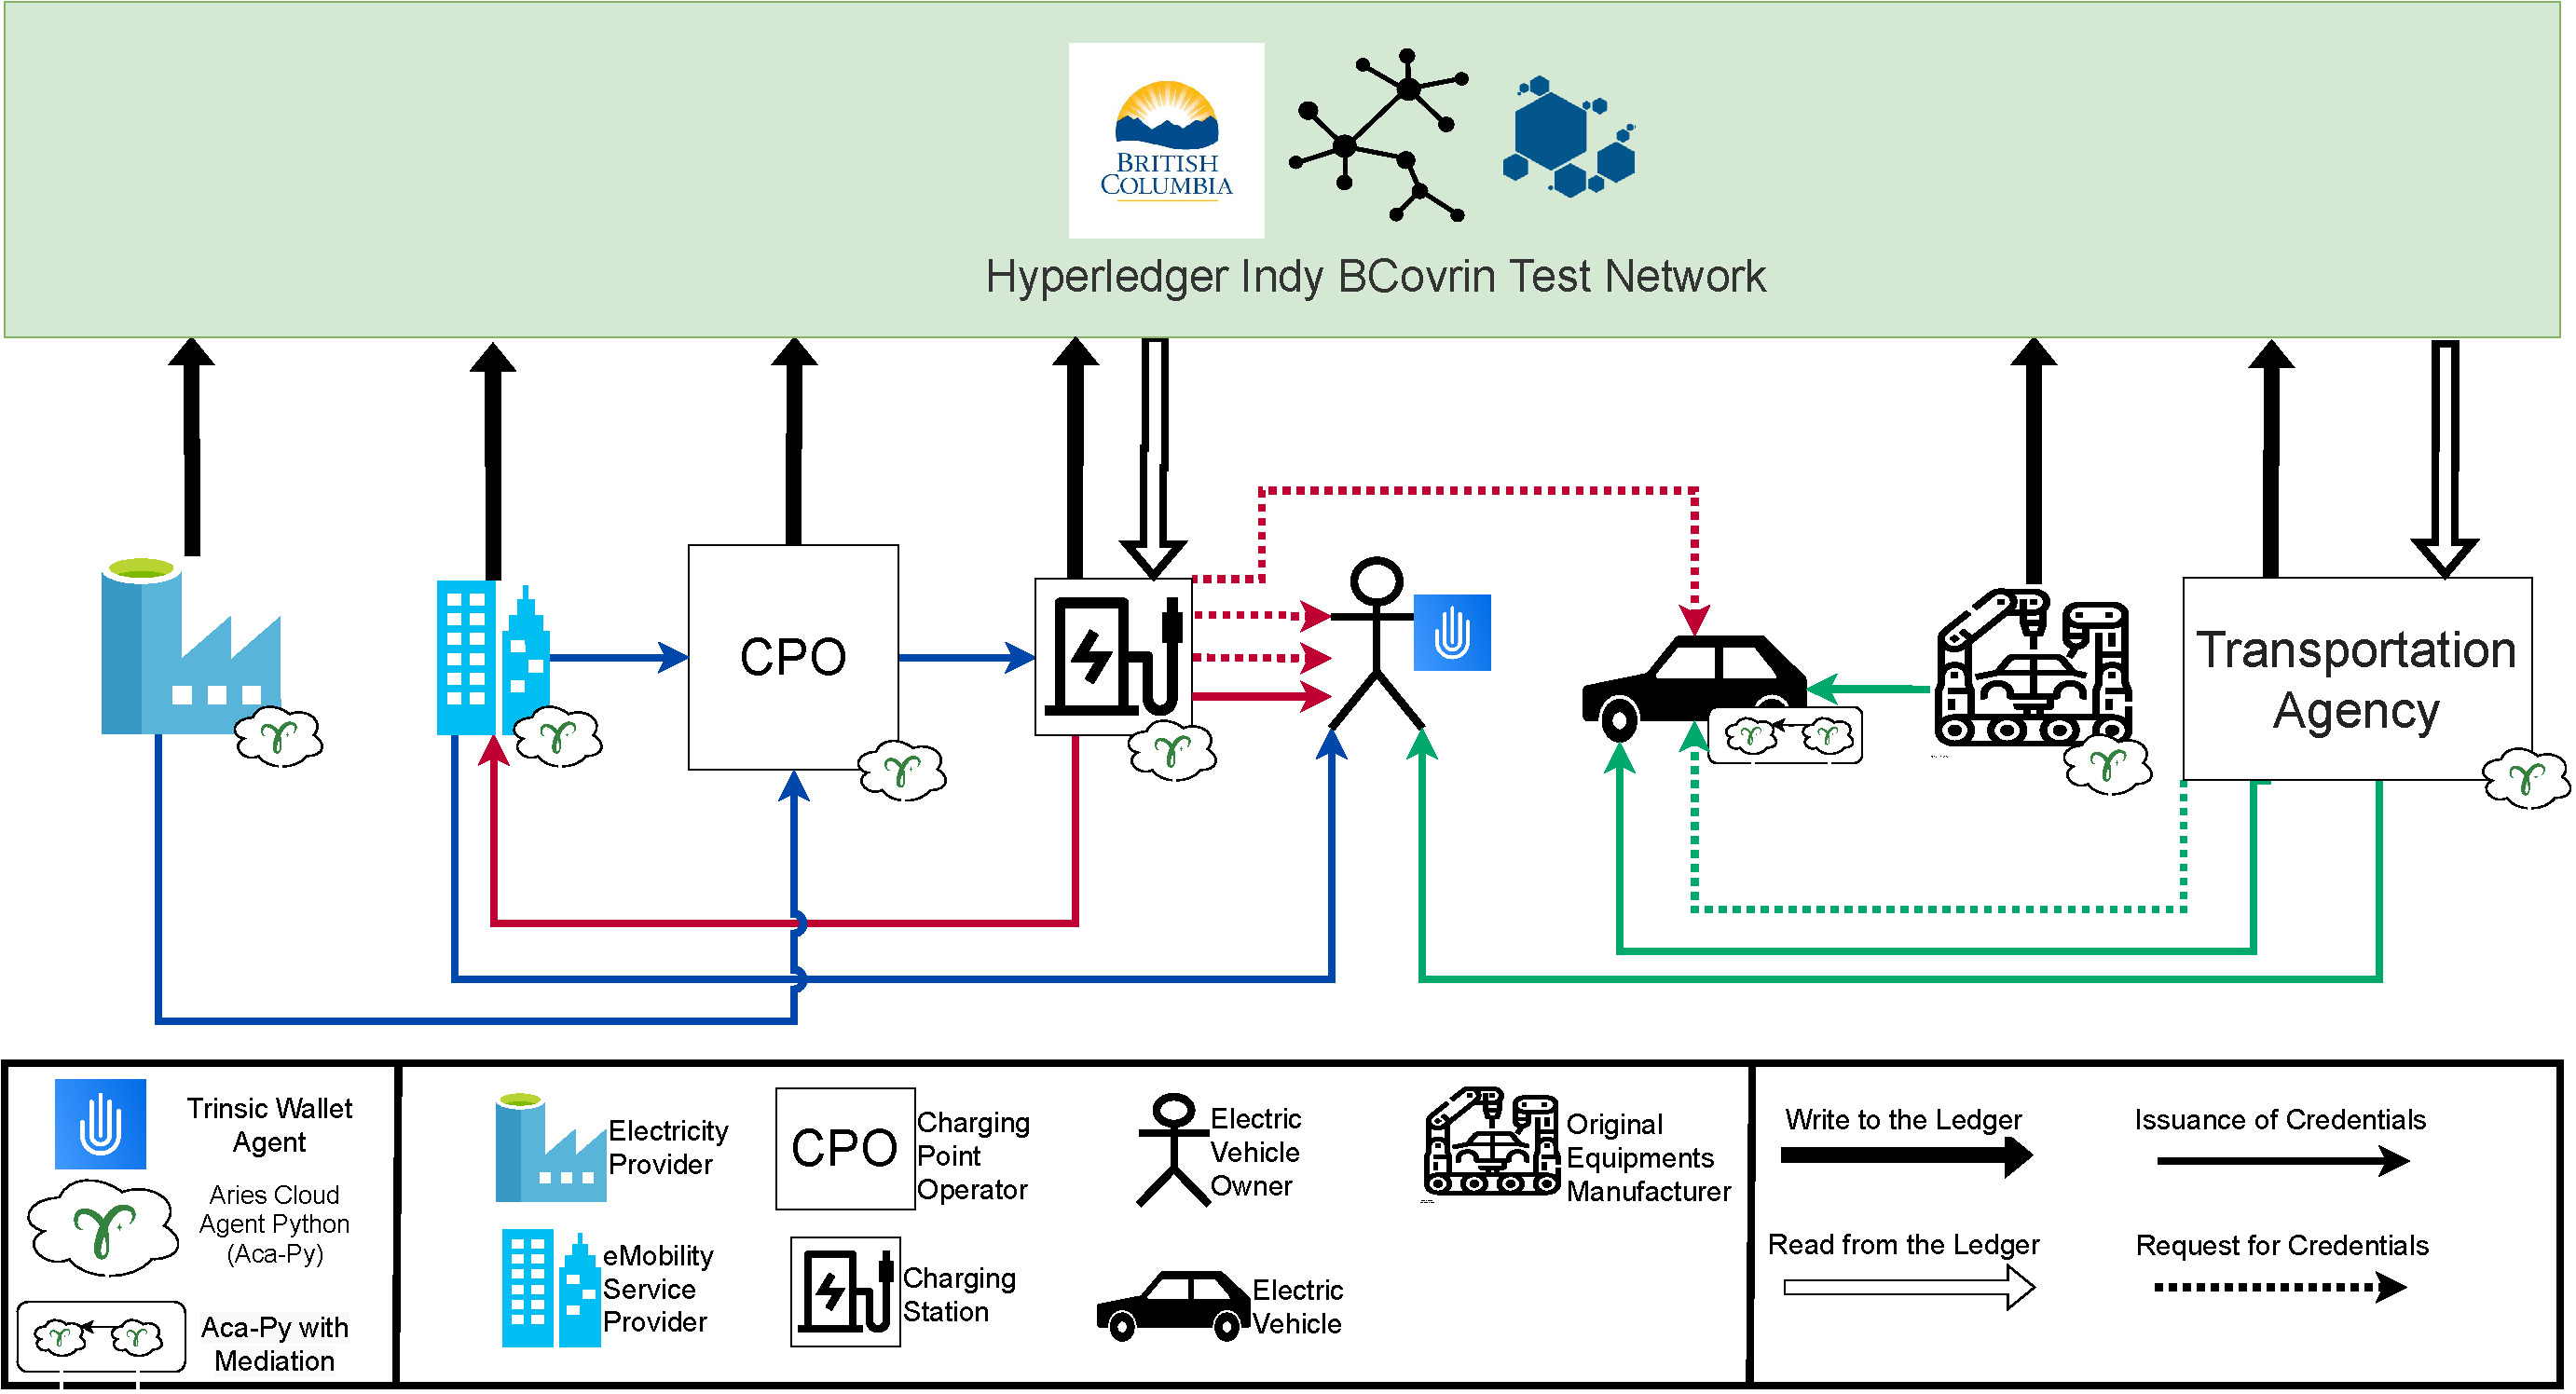
\includegraphics[width=\linewidth]{images/PaperHighLevelArchitecture.pdf}
    \caption{High-Level Architecture Electric Vehicle Charging System with SSI}
    \label{fig:High-Level_Architecture_SSI}
\end{figure}

\subsubsection{Architecture of the System}
\label{subsubsec:architecture_of_the_system}

In Figure~\ref{fig:High-Level_Architecture_SSI} a high-level architecture diagram of the Electric Vehicle Charging System with SSI is demonstrated. This diagram highlights the interactions between each party and between the parties and the Hyperledger Indy Network.

\paragraph{Agents}

Adding Agents to the parties listed in Section~\ref{subsubsec:users_and_information_flows}, and also including the Indy Distributed Network which implements the DLT are the first steps to migrate to the new architecture.
Each party in this diagram represents a group of entities, which will have one agent each. For the sake of simplification, in the diagram presented in Figure~\ref{fig:High-Level_Architecture_SSI} only one of each entity is displayed. 

All parties except the EV Owner are bearers of an ACA-Py, following the choices made in Section~\ref{subsubsec:agent_technology}. All of these ACA-Py agents need to be registered to the network (listed in Section~\ref{subsubsec:distributed_Ledger}) in order to be successfully deployed/started.
Although all agents except the EV Owners are running the ACA-Py agent, they are not all configured the same.
The EV is considered to be an entity whose identity and details should remain anonymous, similarly to the EV Owner. In these two instances (the EV and EV Owner) no public DIDs should be written to the ledger, in order to preserve privacy. 
In the case of the EV running the ACA-Py agent, the difference from the other parties is that no Public DID is registered to the network, and that way no other agent on the ledger will know how to connect to this EVs agent.

The EV Owner's agent is meant to be used as a personal device agent, hence the usage of the Trinsic Wallet Mobile App (available on the App Store and Google Play Store). This agent offers an easy-to-deploy scenario for users, without the need for any additional configurations on the developer or end-user end. This agent, as mentioned previously, is allowed to interact with the BCovrin Test Network without a Public DID. This allows for greater privacy since no details are written onto the ledger.

Following the introduction of the ACA-Py agents in Section~\ref{subsubsec:agent_technology}, and in order to provide a better understanding of the capabilities of the agents and how these can be used independently of the use case, an example of how to use the primary REST endpoints exposed by the agent implementation is presented below. 
In order for an entity agent to issue a credential to another agent, it is first necessary to create a \textit{credentialJSON} object following the specification provided in the agents documentation, and then perform a POST request to the agents endpoint using the following format:

\begin{lstlisting}[language=Bash]
    curl -XPOST -H "Content-type: application/json" -d '{credentialJSON}' 'issuerAgentEndpoint/issue-credential/send'
\end{lstlisting}

Since the implementation of the proposed solution makes use of the automation offered by the agents (by tweaking the deployment parameters, explained later in the deployment chapter), the flow of issuing a credential from one agent to another is automated after the first POST call is made (marked in the above snippet of the script as 'issuerAgentEndpoint/issue-credential/send'). Therefore, none of the other REST endpoints regarding accepting the credential or storing it in the entities' wallet is needed as this is done automatically by the agents.

\paragraph{Mediation}

Given that the EV and the EV Owners agents should not have public DIDs and therefore do not have endpoints to connect to, brings the need for mediation in the proposed solution, a term already introduced in Section~\ref{subsubsec:agent_technology}. 

For the EV agent mediation, another ACA-Py agent is deployed whose purpose is to act solely as a mediator for one EV agent. This mediation can be established during the deployment of each EV agent. Mediation is already implemented under-the-hood for the EV Owner, running the Trinsic Wallet agent, given that the latter handles mediation internally. 

This way, the connections established between the EV Owner/EV and their respective mediators, as well as the mediators with all other agents is end-to-end encrypted, preserving the privacy of the EV Owner and EV and allows them to receive messages later, if offline.

\paragraph{Network Roles and fees}

Given that the proposed solution uses a test network, there are no costs related to performing any actions. But, in a production environment, writing information to the ledger may cost money (for example Sovrin charges \$50 to write a Schema\footnote{\url{https://sovrin.org/issue-credentials/}} to its production network). In Figure~\ref{fig:High-Level_Architecture_SSI} this information regarding who writes to the ledger is marked with the lines going to the Hyperledger Indy BCovrin Test Network, which essentially marks the entities that in a production level network would need to pay fees.

\paragraph{Distributed Ledger}

The Distributed Ledger is responsible for storing the Public DIDs of issuing or mediator agents, and information regarding the schemas and credential definitions. Additionally it contains information about the revocation registries, so that revocation can be allowed in this system.
Every time an agent wishes to issue a new credential type to another agent, it needs to hold a credential definition previously written to the ledger, stating that it can issue credentials to others under a set of attributes defined in a linked schema (this schema may be issued by the same agent or a different one). From that point on, that agent is authorized to issue credentials under that credential definition.

\paragraph{Revocation Registry}

The revocation registry is used as a means to provide revocation to the credentials. It is not inherently included in the deployed network, but it is a component whose purpose is relevant together with an Hyperledger Indy network, hence this was abstracted in Figure~\ref{fig:High-Level_Architecture_SSI} and included it in the "Hyperledger Indy BCovrin Test Network". When a credential definition is created, and when the revocation flag is set to \textit{true}, a revocation registry will automatically be created, and a tails file will be uploaded to the revocation registry (also named as tails server). Revoking credentials is made the same way as issuing a credential, in the way that these actions are handled by the agents by means of REST APIs. When an agent wishes to revoke a credential that was previously issued, it adds a revocation registry entry to the tails server indicating the revocation of a given credential, so that verifiers can look up the credential on the tails server and validate whether the credential is still valid.

\subsubsection{Schemas and Credential Definitions}
\label{subsubsec:schemas_and_CDs}

One of the main goals of transposing the architecture of the current paper-based model to the SSI-powered system is to port credentials into VCs. These can be credentials that attest signed contracts, ownership attestations, legal documentation, etc. In this system there are a number of exclusive parties that will be allowed to create schemas and credential definitions, which will be used as the template to issue credentials to the remaining parties. After dissecting the problem and understanding where it is possible to create and adapt VCs, the following mapping listed in Table~\ref{tab:mapping_of_credentials} has been made.

\begin{table}[!htb]
    \begin{tabularx}{\linewidth}{|c|c|c|X|} 
    \hline
    \textbf{Credential ID} & \textbf{Schema and CD Issuers} & \textbf{Target Holders} & \textbf{Verbose} \\
            \hline
            1 & OEM & EV & Credential containing information on the EVs' VIN. \\
            \hline
            2 & TA & EV & Credential attesting the EV is registered and allowed to be driven on the streets. \\
            \hline
            3 & TA& EV Owner & Credential attesting that the EV Owner is allowed to drive the EV they possess. \\
            \hline 
            4 & eMSP & EV Owner & Credential representing signed contract between eMSP and EV Owner. \\
            \hline
            5 & eMSP & CPO & Credential representing signed contract between eMSP and CPO. \\
            \hline
            6 & CPO & CS & Credential attesting that a specific CS is owned by the respective CPO. \\
            \hline
            7 & CS & EV Owner \& eMSP & Credential containing receipt of charging transaction. \\
            \hline
            8 & EP & CPO & Credential representing signed contract between EP and CPO. \\
            \hline
    \end{tabularx}
    * For the sake of the proposed solution, the issuers of the schemas are the parties who issue said credentials. In a production environment these schemas can be issued by Governmental Parties or Domain-Regulatory Parties, in order to ensure interoperability between all the different vendors.
    \caption{Mapping of Paper-Based Credentials to Verifiable Credentials}
    \label{tab:mapping_of_credentials}
\end{table}

The attributes of the most important credentials in Table~\ref{tab:mapping_of_credentials} are listed below. More fields can be added to the credentials, allowing these to be used for other use cases and applications.

\begin{itemize}
    \item \textbf{Credential 1}
    \begin{itemize}
        \item VIN - The VIN number is used by the TA in order to validate that the EV is registered with a valid number by the OEM.
    \end{itemize}
    \item \textbf{Credential 2 and 3}
    \begin{itemize}
        \item registrationID - This registrationID is the link between the EV and its EVOwner, since both hold the same registrationID.
    \end{itemize}
    \item \textbf{Credential 4}
    \begin{itemize}
        \item eMSPcontractID - This contractID is used in the charging process as an identifier of the EVOwner to a contract that is valid, provided by the eMSP.
    \end{itemize}
    \item \textbf{Credential 7}
    \begin{itemize}
        \item kWh - This attribute holds the information regarding the price per kWh at the time of charging.
        \item Price - This attribute holds the information regarding the price of the charging transaction.
        \item eMSPContractID - This attribute is used to link transactions to a specific eMSPContractID (Credential 4).
    \end{itemize}
\end{itemize}

\subsubsection{Information Flows with SSI}
\label{subsubsec:information-flows-ssi}

In this section the different flows highlighted in Section~\ref{subsec:case_description} and how they are handled in the new system will be discussed, marking the similarities between the previous architecture and the proposed architecture with SSI, while also explaining the state of the wallet of the agents after each flow.

\paragraph{Service Providers Flow with SSI}
\label{paragraph:service_providers_flows_with_ssi}

In order for the system to be operational for authentication of EV Owners and charging of the EVs, credentials \#4, \#5, \#6 and \#8 need to be present upon the systems initial configuration. In the original architecture, an EV Owner needs to hold a contract with an eMSP in order to be allowed to charge the EV, for example. Other details about each credential and their purpose will be explained in-depth with each use case description. During this flow, credentials will only be issued from one party to another without any previous credential verification (at least with the current assumptions made). It is important to mention that the interactions in Figure~\ref{fig:High-Level_Architecture_SSI} with the \textcolor{blue}{\textbf{Blue Lines}}, correspond to the information provided in the \textbf{Service Providers} flow in Section~\ref{subsubsec:users_and_information_flows}. 

Before making this analysis, there are a number of assumptions that need to be made:

\textit{The EVOwner has a contract signed with the respective eMSP and the details have been agreed on by both parties in the physical world.}

Table~\ref{tab:roles_of_service_providers} highlights the parties and their respective roles (Issuer, Holder, Verifier and/or Trusted Party) in this particular flow.

\begin{table}[H]
    \centering
    \begin{tabular}{|c|c|c|c|c|}
        \hline
        \backslashbox{Party}{Role} & Issuer & Holder & Verifier & Trusted Party \\\hline
        eMSP & \checkmark &  & & \\
        Charging Point Operator & \checkmark & \checkmark & & \\
        Charging Station & & \checkmark & & \\
        Electricity Provider & \checkmark & & & \\
        EV Owner & & \checkmark & & \\
        \hline
    \end{tabular}
    \caption{Roles of the parties involved in the "Service Providers Flow"}
    \label{tab:roles_of_service_providers}
\end{table}

In this flow, the steps of the communication are represented in the System Sequence Diagram in Figure~\ref{fig:service_providers_ssd}. Note that given that this flow incorporates four different use cases, that are not dependent on each other, these have been separated both in the figure as well as in the description below, but can be performed in no particular order.

\begin{itemize}
    \item Use Case "EVOwner/eMSP"
    \begin{enumerate}
        \item eMSP: The interaction between the eMSP and the EVOwner should begin by the eMSP generating a connection invitation in the form of a QR Code using the HTTP endpoints provided by the agent. 
        \item EVOwner: The user scans the QR Code using the Trinsic Wallet App, and accepts the connection invitation. After this point the two agents are connected via a pairwise-DID channel.
        \item eMSP: The eMSP will then proceed to issue a "Contract between eMSP and EVOwner" (Credential \#4) credential to the EVOwner.
    \end{enumerate}
    \item Use Case "eMSP/CPO"
    \begin{enumerate}
        \item eMSP: The eMSP agent will send out a connection request to the CPO agent.
        \item CPO: The CPO agent accepts the connection request and after this point the two agents are connected via a pairwise-DID channel.
        \item eMSP: The eMSP will issue a "Contract between eMSP and CPO" (Credential \#5) to the CPO agent.
    \end{enumerate}
    \item Use Case "EP/CPO"
    \begin{enumerate}
        \item EP: The EP agent will send out a connection request to the CPO agent.
        \item CPO: The CPO agent accepts the connection request and after this point the two agents are connected via a pairwise-DID channel.
        \item EP: The EP will issue a "Contract between EP and CPO" (Credential \#8) to the CPO agent. 
    \end{enumerate}
    \item Use Case "CPO/CS"
    \begin{enumerate}
        \item CPO: The CPO agent will send out a connection request to the CS agent.
        \item CS: The CS agent accepts the connection request and after this point the two agents are connected via a pairwise-DID channel.
        \item CPO: The CPO will issue a "Ownership of CS" (Credential \#6) to the CS agent. 
    \end{enumerate}
\end{itemize}

During the "Service Providers" flow the mentioned agents should receive the following credentials in their wallets:
\begin{itemize}
    \item EV Owner Agent Wallet
        \begin{enumerate}
            \item Credential (\#4) with Contract information with eMSP
        \end{enumerate} 
    \item CPO Agent Wallet
        \begin{enumerate}
            \item Credential (\#5) with Contract information with eMSP
            \item Credential (\#8) with Contract information with EP
        \end{enumerate}
    \item CS Agent Wallet 
        \begin{enumerate}
            \item Credential (\#6) with Proof of Ownership from CPO
        \end{enumerate}
\end{itemize}

\begin{figure}[!h]
    \centering
    \frame{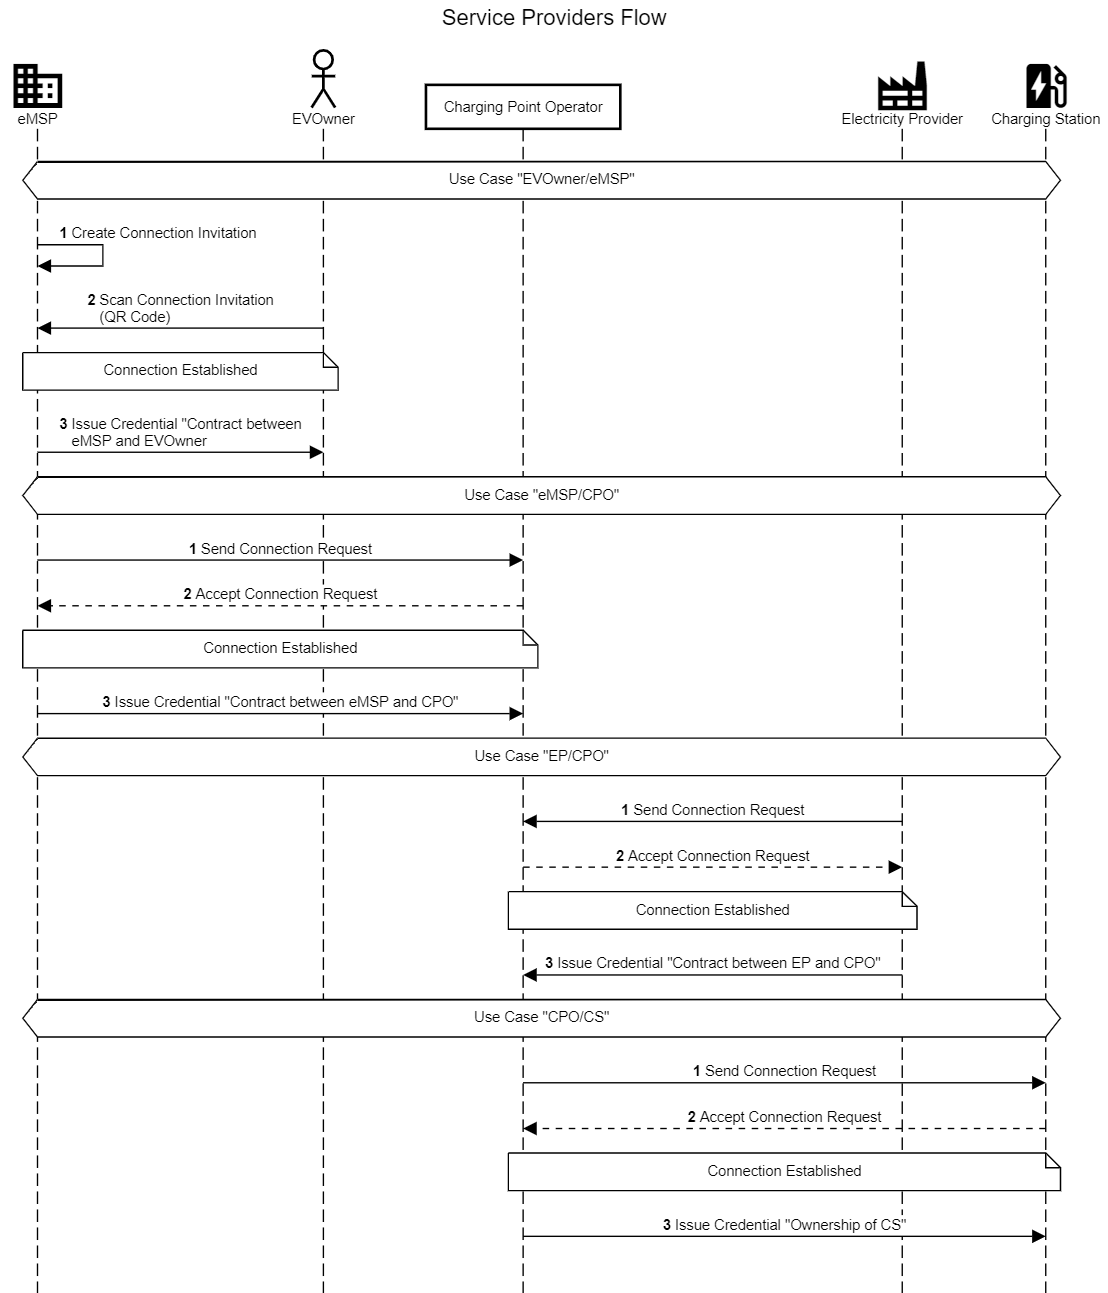
\includegraphics[keepaspectratio=true,width=0.85\textwidth]{images/SSDs/Service_Providers_Flow.png}}
    \caption{Service Providers Flow System Sequence Diagram}
    \label{fig:service_providers_ssd}
\end{figure}

\newpage

\paragraph{EV Owner and EV Interactions with SSI}
\label{paragraph:ev_owner_and_ev_interactions_with_ssi}

The \textbf{EV Owner and EV Interactions} flow is ported over to the new system with the usage of the interactions marked with the \textcolor{green}{\textbf{Green Lines}} in Figure~\ref{fig:High-Level_Architecture_SSI}. This is the first part of the system that requires credential verification. It starts with the EV being issued a VIN by the OEM through means of a credential. After that, the EV is meant to be registered by the local TA (for example the RDW in the Netherlands) and should be given a credential to attest this process. The EV Owner will need to confirm with the TA that it owns the EV it wishes to register; this could be perceived as a credential to add in the future to the system, so in order to simplify this portion of the system an assumption is made that the EV Owner is able to present a credential to this effect. After this, the TA issues a credential to the EV Owner with matching information that can link the EV Owner and its EV (for example the registration ID present in both credentials).

Before making this analysis, there are a number of assumptions that need to be made:
\begin{itemize}
    \item \textit{The OEM is the party that creates the vehicle, hence it can manually operate and deploy the EVs agent and establish a connection to it.}
    \item \textit{The EVOwner has a proof of purchase that is sent to the TA which entitles it to register the EV in their name.}
    \item \textit{The EV Owner and the EV will hold the same registration ID in their credentials given out by the TA, in order to link the two.}
\end{itemize}

Table~\ref{tab:roles_ev_and_ev_owner_interactions} highlights the parties and their respective roles (Issuer, Holder, Verifier and/or Trusted Party) in this particular part of the use case.

\begin{table}[H]
    \centering
    \begin{tabular}{|c|c|c|c|c|}
        \hline
        \backslashbox{Party}{Role} & Issuer & Holder & Verifier & Trusted Party \\\hline
        EV & & \checkmark & & \\
        EV Owner & & \checkmark & & \\
        TA & \checkmark & & \checkmark & \\
        OEM & \checkmark & & & \checkmark \\
        \hline
    \end{tabular}
    \caption{Roles of the parties involved in the "EV Registration and EV Ownership Registration" use case}
    \label{tab:roles_ev_and_ev_owner_interactions}
\end{table}

In this Information Flow, the steps of the communication are represented in the System Sequence Diagram in Figure~\ref{fig:ev_and_ev_owner_interactions_ssd}:

\begin{enumerate}
    \item EV: The flow commences with the EV sending a connection request (previously generated) to the OEM agent.
    \item OEM: The OEM receives the invitation and accepts it, establishing a pairwise-DID connection between the two agents.
    \item OEM: The OEM agent now issues a "Vehicle VIN" (Credential \#1) credential to the EV agent.
    \item EV: The EV agent now wishes to connect to the TA agent, sending a connection request to the latter.
    \item TA: The TA agent receives the connection request and accepts it, establishing a pairwise-DID connection between the two agents.
    \item TA: The TA agent now requests the "Vehicle VIN" credential from the EV, which was issued previously by the OEM (Credential \#1). It requests the VIN attribute and whether the expiration date is greater than the current date.
    \item EV: The EV receives the presentation request and generates a proof presentation using the credential issued by the OEM earlier.
    \item EV: The EV now sends the proof presentation to the TA agent.
    \item TA: The TA agent receives the proof, verifies it and proceeds to send an "EV Registration" (Credential \#2) credential to the EV.
    \item TA: The interaction between the TA and the EVOwner should begin by the TA generating a connection invitation in the form of a QR Code using the HTTP endpoints provided by the agent. 
    \item EVOwner: The user scans the QR Code using the Trinsic Wallet App, and accepts the connection invitation. After this point the two agents are connected via a pairwise-DID channel.
    \item TA: An event which is not contemplated in the PoC is the agent holding a credential to attest proof of purchase of the EV to register it. But in an ideal scenario the TA agent requests a "Proof of Purchase" credential from the EVOwner.
    \item EVOwner: The EVOwner receives the presentation request and generates a proof presentation with the "Proof of Purchase" credential (which is an assumption and is not contemplated in this PoC, as previously stated).
    \item EVOwner: The EVOwner now sends the proof presentation to the TA agent.
    \item TA: At last, the TA agent issues an "EV Owner Registration" (Credential \#3) credential to the EVOwner.
    
\end{enumerate}

\begin{figure}[!]
    \centering
    \frame{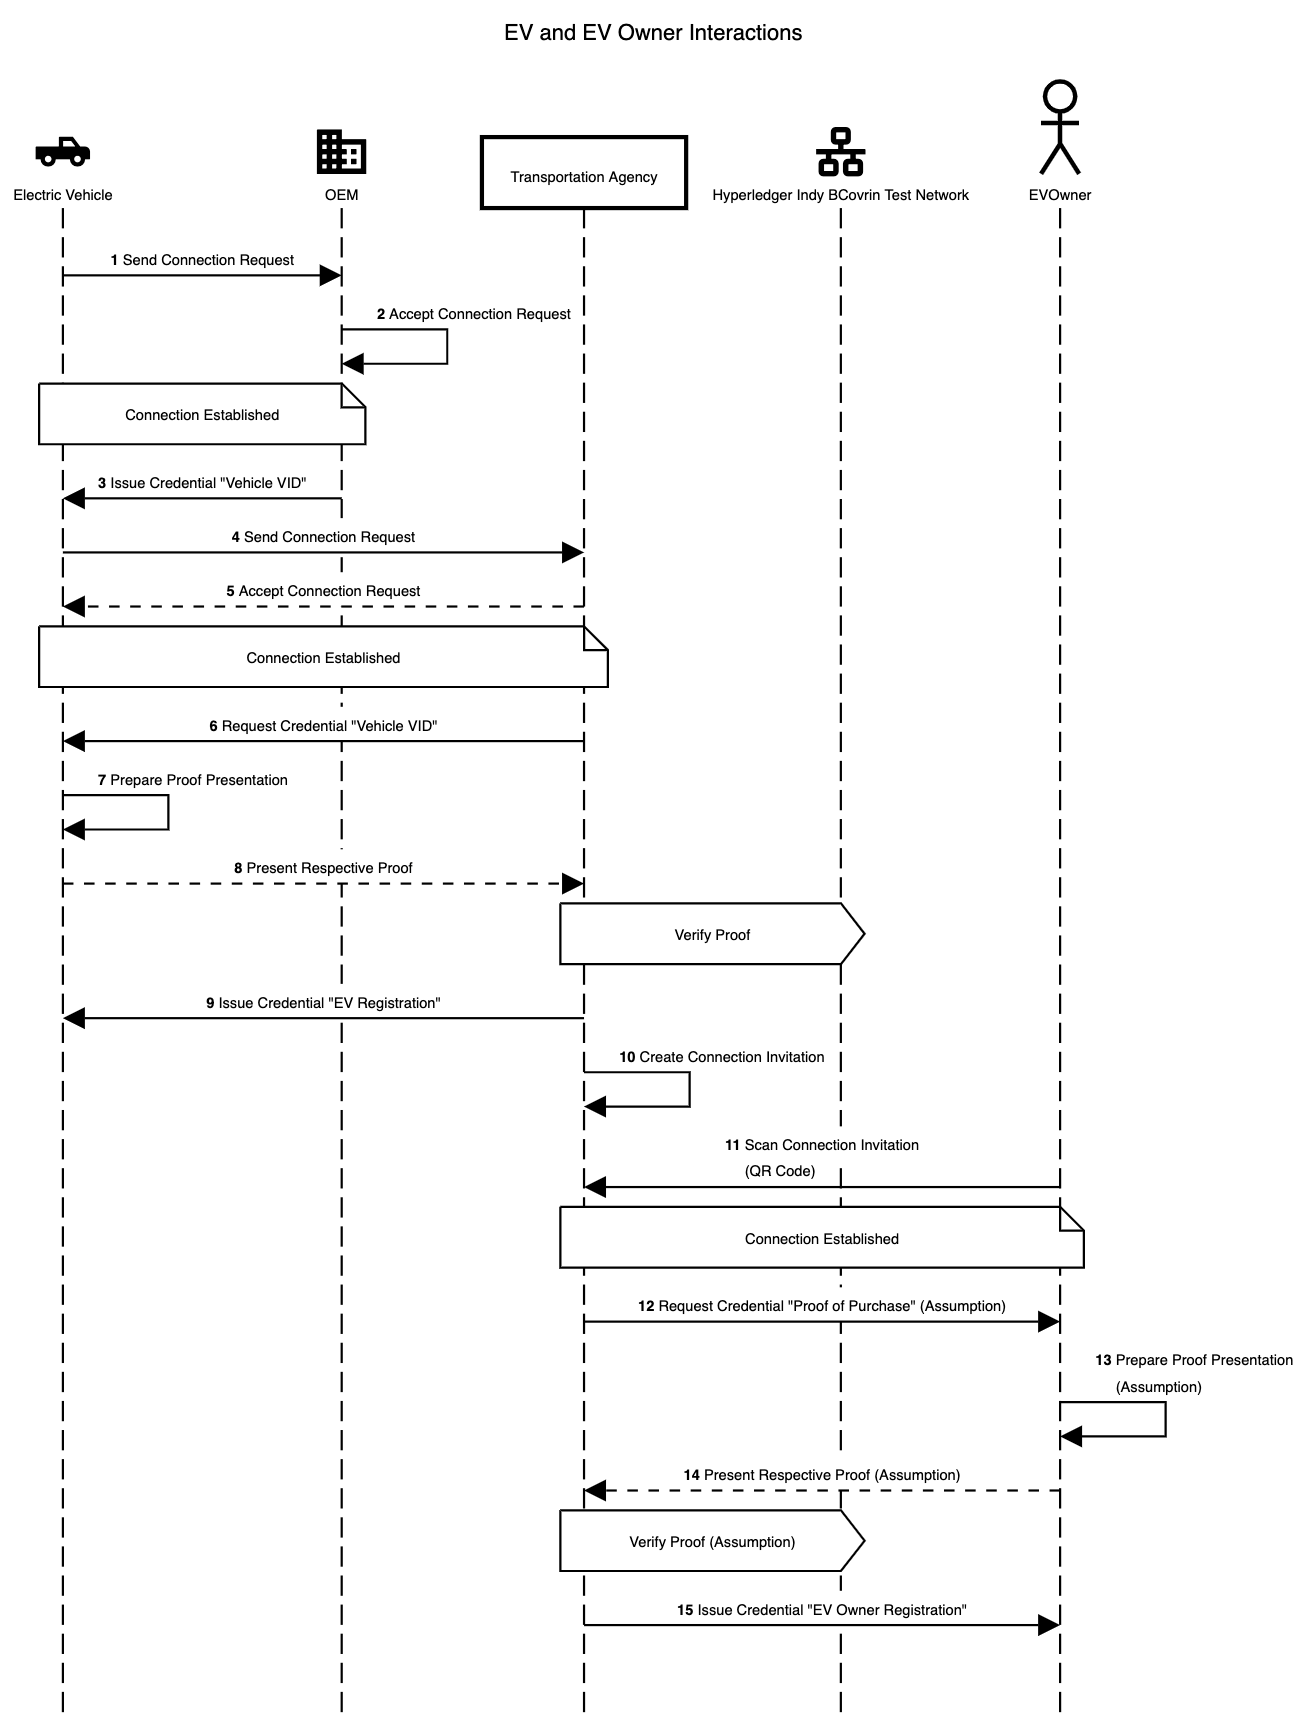
\includegraphics[keepaspectratio=true,width=\textwidth]{images/SSDs/EV_and_EV_Owner_Interactions.png}}
    \caption{EV and EV Owner Interactions System Sequence Diagram}
    \label{fig:ev_and_ev_owner_interactions_ssd}
\end{figure}

During the "EV Owner and EV Interactions" flow the mentioned agents should receive the following credentials in their wallets:

\begin{itemize}
    \item EV Agent Wallet
    \begin{enumerate}
        \item Credential (\#1) with Vehicle VIN from OEM
        \item Credential (\#2) with EV Registration from TA 
    \end{enumerate}
    \item EV Owner Agent Wallet 
    \begin{enumerate}
        \item Credential (\#3) with EV Owner Registration from TA
    \end{enumerate}
\end{itemize}

\paragraph{Charging and Billing Flow with SSI}
\label{paragraph:charging_and_billing_flow_with_ssi}

The most important part of this system is exactly demonstrating how to improve the privacy of the act of charging the EV; additionally, the system with SSI aims to tackle one of the key issues with the previous architecture: to provide means for the users to know the kWh rate, hence giving the opportunity to deny charging if the rate is too high according to the users desire. Additionally, it is also important to introduce in the system a way for the user to know how much they have spent after each charging session, and keep a record of that.
For this, the proposed architecture aims at the end of each transaction to give power to each Charging Station agent to issue a credential to the EV Owner with a "receipt-like" credential, that can be used later to prove claims and also to the eMSP to prove that a specific user has charged its vehicle (seen with the \textcolor{red}{\textbf{Red Lines}} in Figure~\ref{fig:High-Level_Architecture_SSI}). In order for EV Owners to know the rate at which the EV will be possibly charged, the Charging Station agent shall communicate with the CPO agent to obtain this information, and pass it on as a DIDComm Basic Message\footnote{\url{https://github.com/hyperledger/aries-rfcs/tree/527849ec3aa2a8fd47a7bb6c57f918ff8bcb5e8c/features/0095-basic-message}}.

Before making this analysis, there are a number of assumptions that need to be made:

\textit{The connection between the Charging Station and the EV is simplified since the process to send information from an EV to a CS falls out of the scope of this study. The reason is that the domain-specific protocols are not easy to integrate in this solution and need to be better assessed in the future.}

Table~\ref{tab:roles_of_charging_and_billing} highlights the parties and their respective roles (Issuer, Holder, Verifier and/or Trusted Party) in this particular part of the use case.

\begin{table}[H]
    \centering
    \begin{tabular}{|c|c|c|c|c|}
        \hline
        \backslashbox{Party}{Role} & Issuer & Holder & Verifier & Trusted Party \\\hline
        Charging Station & \checkmark & & \checkmark & \\
        EVOwner & & \checkmark & & \\
        Electric Vehicle & & \checkmark & & \\
        eMSP & & \checkmark & & \checkmark \\ 
        Transportation Agency & & & & \checkmark \\
        \hline
    \end{tabular}
    \caption{Roles of the parties involved in the "Charging and Billing Flow"}
    \label{tab:roles_of_charging_and_billing}
\end{table}

In this use case, the steps of the communication are represented in the System Sequence Diagram in Figure~\ref{fig:charging_and_billing_ssd}.

The steps are explained in detail in the following list:

\begin{enumerate}
    \item CS: The interaction should begin by the EV Owner arriving at a Charging Station, that will generate a connection invitation in the form of a QR Code using the HTTP endpoints provided by the agent. 
    \item EVOwner: The EVOwner scans the QR Code using the Trinsic Wallet App, and accepts the connection invitation. After this point the two agents are connected via a pairwise-DID channel.
    \item CS: The Charging Station agent will then request the credential attributes from the EVOwner that prove they hold a contract with an eMSP (Credential \#4).
    \item EVOwner: The EVOwner receives a credential presentation request on the Trinsic Wallet App, and assuming it agrees to disclose the information regarding "Contract ID", "eMSP Company Name" and use ZKP to prove that the "Expiration date of the contract" is greater than the current date, the Trinsic Wallet App will automatically fetch all the relevant attributes from the stored credentials and generate the proof.
    \item EVOwner: The Trinsic Wallet App then submits this proof and sends it back to the CS agent, with a reference to the Credential Exchange ID created by the CS agent in Step 3.
    \item CS: The CS agent receives the proof and verifies it, checking the revocation status of the presentation.
    \item CS: The same process of Steps 3-6 is repeated for the credentials that attest the EV Ownership from the EVOwner, previously issued by the TA (Credential \#3).
    \item CS: In case the EVOwner has a valid contract with an eMSP, the CS will proceed to contact the CPO agent and request the price per kWh for a user contracted under that eMSP, since this can vary depending the contracts signed between the CPOs and the eMSPs. Otherwise the charging session is rejected.
    \item CPO: The CPO agent will receive the message from the CS agent and reply accordingly with a charging rate.
    \item CS: The CS will receive the message and present this information to the EVOwner on the CS dashboard.
    \item CS: The CS will now connect to the EV in order to compare the credential attributes from the EV Owner and the EV and validate they are indeed linked.
    \item EV: The EV agent will accept the connection request from the CS (Note that this process is an assumption and needs to be studied in depth in the future work).
    \item CS: The same process of Steps 3-6 is repeated for the credentials that attest the EV Registration coming from the EV, issued by the TA (Credential \#2).
    \item CS: The values presented by both the EV and EVOwner are compared, and if they match, the charging session starts. Otherwise the charging session is rejected.
    \item CS: At the end of the charging session the CS issues a credential to the EVOwner and the respective eMSP with a receipt of the charging session (Credential \#7).
\end{enumerate}

\begin{figure}[!]
    \centering
    \frame{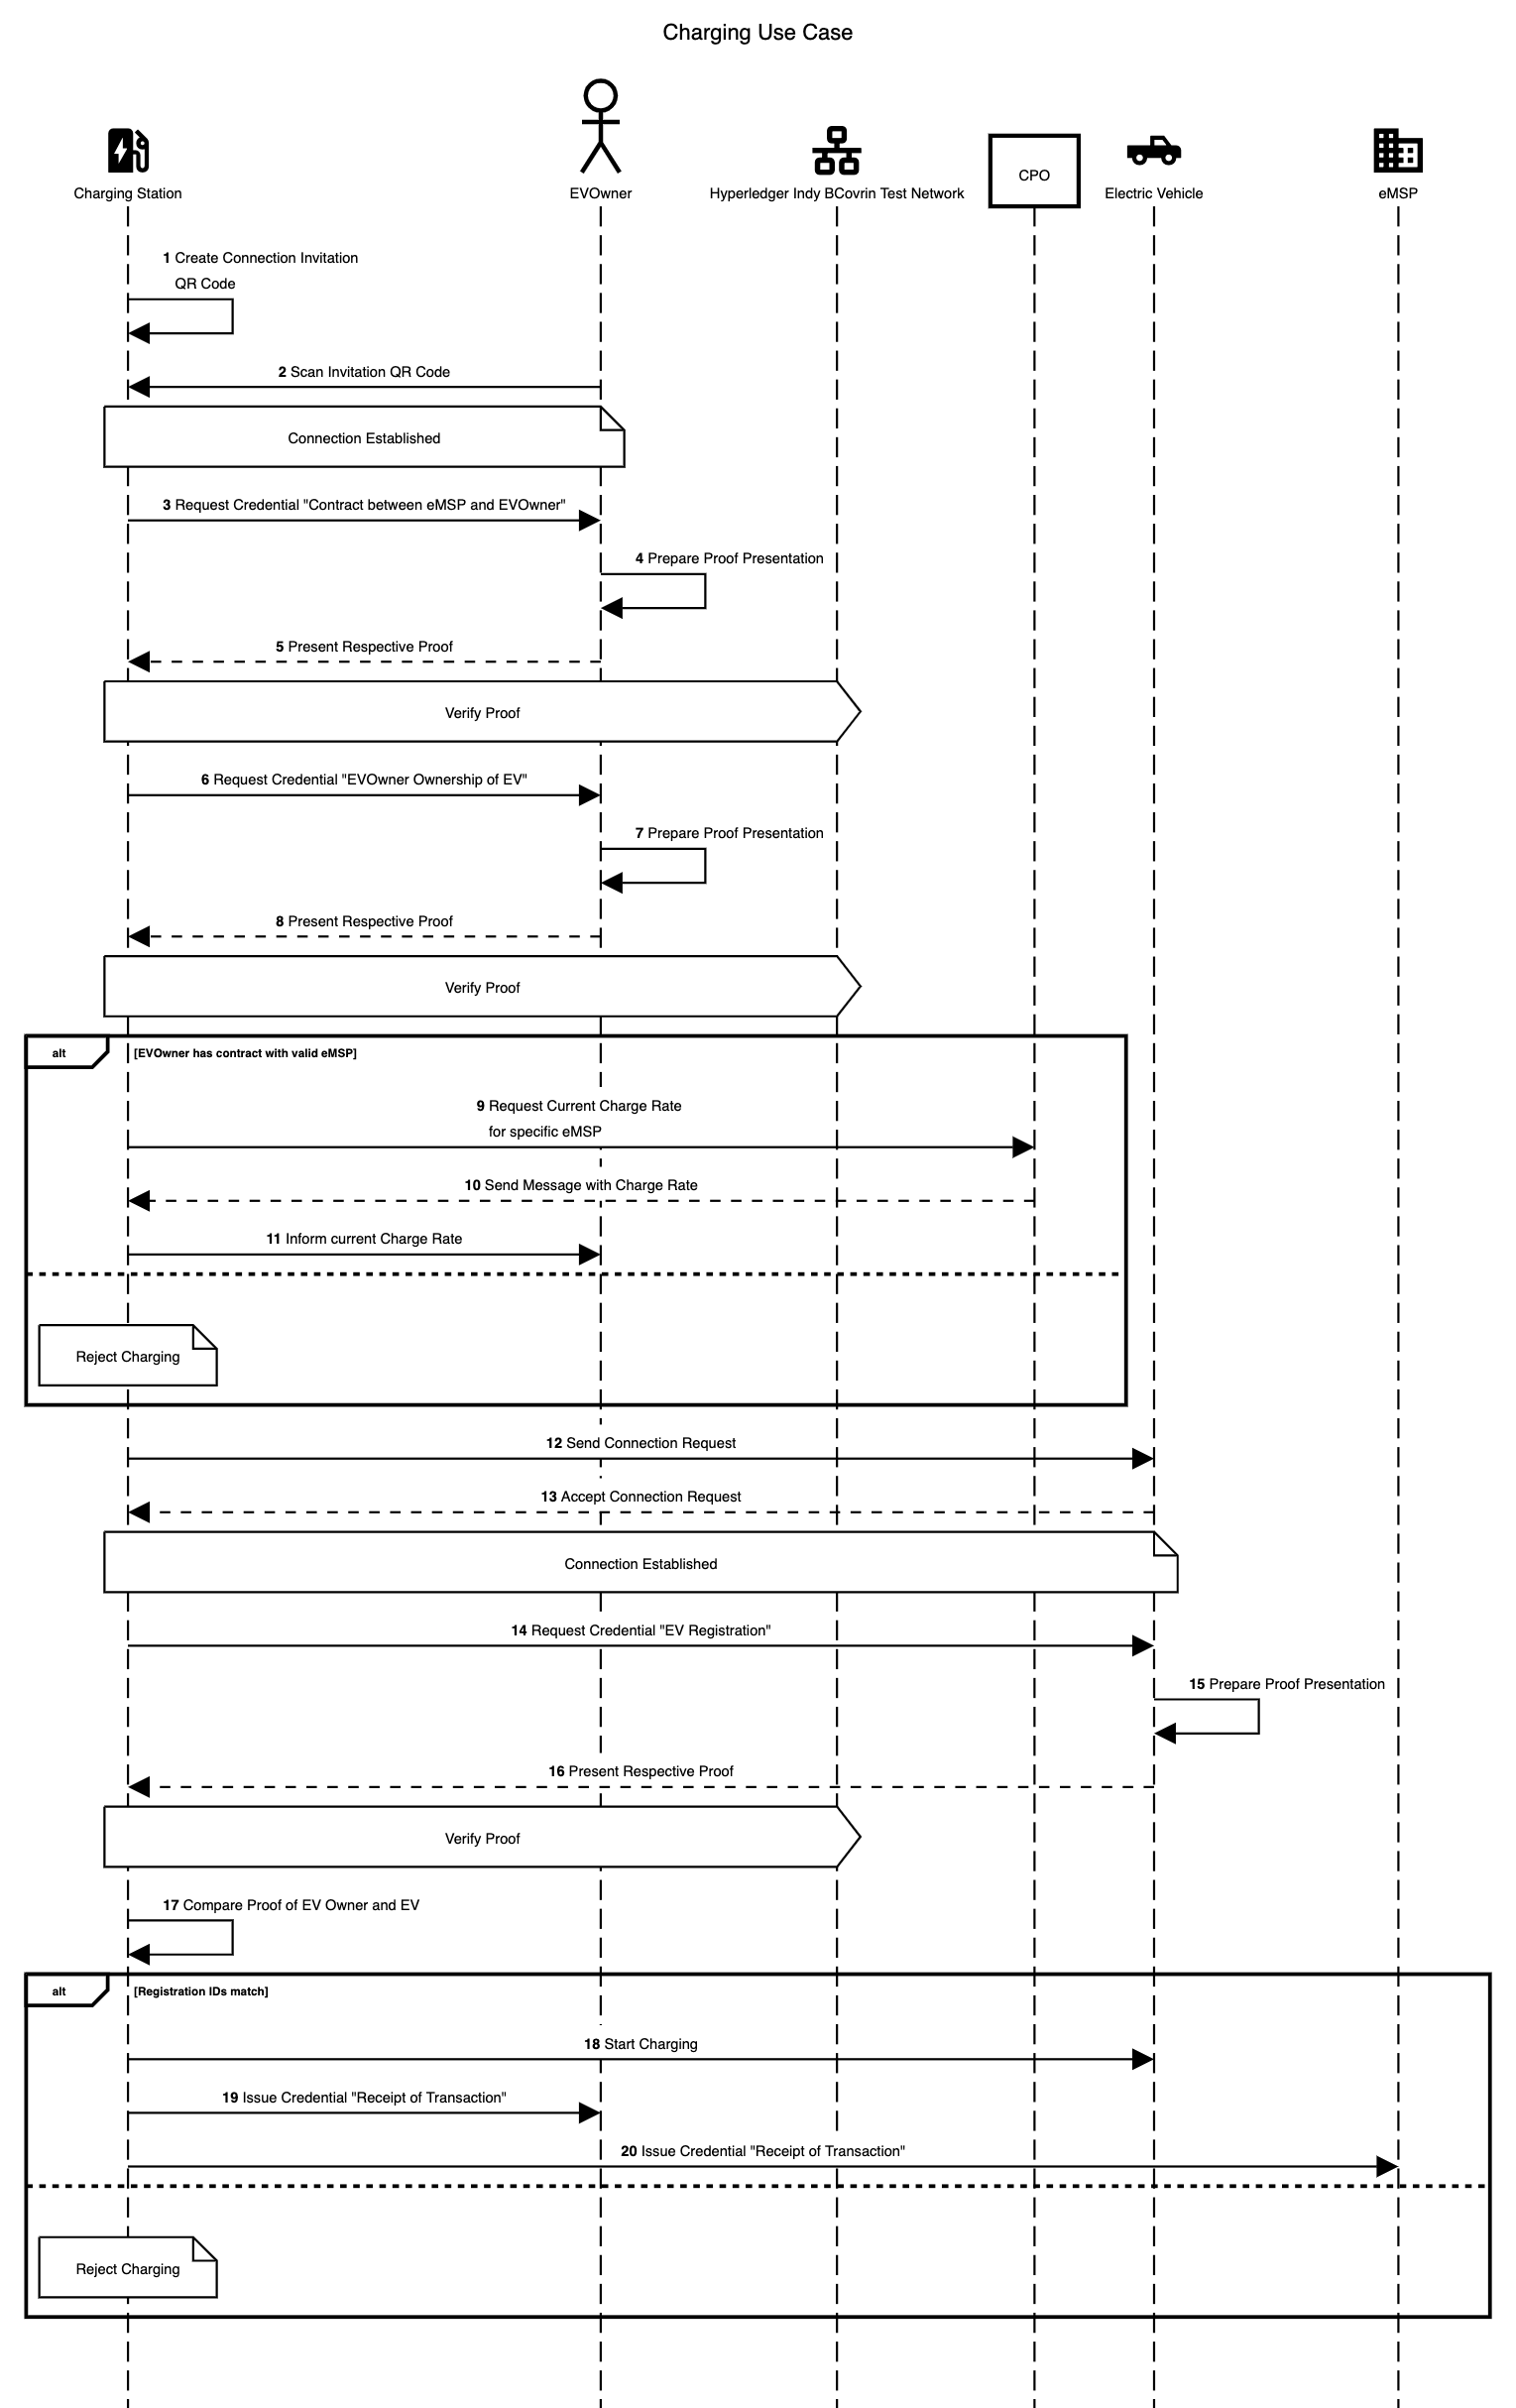
\includegraphics[keepaspectratio=true,height=\textheight]{images/SSDs/Charging_SSD.png}}
    \caption{Charging and Billing Use Case System Sequence Diagram}
    \label{fig:charging_and_billing_ssd}
\end{figure}


During the "Charging and Billing" flow the mentioned agents should receive the following credentials in their wallets:

\begin{itemize}
    \item EV Owner Agent Wallet
    \begin{enumerate}
        \item Credential (\#7) with Receipt of Charging Session from Charging Station
    \end{enumerate}
    \item eMSP Agent Wallet
    \begin{enumerate}
        \item Credential (\#7) with Receipt of Charging Session from Charging Station
    \end{enumerate}
\end{itemize}
